%!Mode:: "TeX:UTF-8"
\documentclass[a4paper,11pt,UTF8]{ctexart}

\usepackage{indentfirst} %缩进
\usepackage{xeCJK}    %使用系统字体
\usepackage{fancyhdr} %自定义页眉页脚
\pagestyle{empty}                   %不设置页眉页脚
\usepackage{amsmath, amsthm, amssymb, amsfonts} %数学公式
\usepackage[a4paper,left=3cm,right=3cm,top=3cm,bottom=3cm]{geometry}
%\usepackage[tmargin=1in,bmargin=1in,lmargin=1.25in,rmargin=1.25in]{geometry}.
\usepackage{booktabs} %插入表格
\usepackage[section]{placeins} %避免浮动
\usepackage{listings} %插入代码
\usepackage{ctex}     %中文宏包
\usepackage[svgnames, table]{xcolor} %彩色表格
\usepackage{algorithm}          %伪代码
\usepackage{algorithmicx}
\usepackage{algpseudocode}
\usepackage{algorithm,algpseudocode,float}
\usepackage{lipsum}
\usepackage{enumitem}           %调整列举环境
\usepackage{url}
\usepackage{fontspec,xunicode}
\usepackage{upgreek}
\usepackage{wrapfig}
\defaultfontfeatures{Mapping=tex-text} %如果没有它,会有一些 tex 特殊字符无法正常使用,比如连字符。

\usepackage{graphicx}
\graphicspath{{imgs/}}

%%%%%%%%%%%%%%%%%%%%%%%%%%%%%%%%%%%%%%%%%%%%%%%%%%%%%%%%%%%%%%%%
% 缩进及行间距
%%%%%%%%%%%%%%%%%%%%%%%%%%%%%%%%%%%%%%%%%%%%%%%%%%%%%%%%%%%%%%%%
\setlength{\parindent}{22pt} %重新定义缩进长度
\setlength{\baselineskip}{20pt}  %定义行间距
%\renewcommand{\baselinestretch}{1.1} %定义行间距

%%%%%%%%%%%%%%%%%%%%%%%%%%%%%%%%%%%%%%%%%%%%%%%%%%%%%%%%%%%%%%%%
% 列表设置
%%%%%%%%%%%%%%%%%%%%%%%%%%%%%%%%%%%%%%%%%%%%%%%%%%%%%%%%%%%%%%%%
\setenumerate{fullwidth,itemindent=\parindent,listparindent=\parindent,itemsep=0ex,partopsep=0pt,parsep=0ex}
\setenumerate[2]{label=\alph*),leftmargin=1.5em}  %二级item设置
\setitemize{itemindent=38pt,leftmargin=0pt,itemsep=-0.4ex,listparindent=26pt,partopsep=0pt,parsep=0.5ex,topsep=-0.25ex}
\setdescription{itemindent=38pt,leftmargin=0pt,itemsep=-0.4ex,listparindent=26pt,partopsep=0pt,parsep=0.5ex,topsep=-0.25ex}

%%%%%%%%%%%%%%%%%%%%%%%%%%%%%%%%%%%%%%%%%%%%%%%%%%%%%%%%%%%%%%%%
% 图的标题行间距设置
%%%%%%%%%%%%%%%%%%%%%%%%%%%%%%%%%%%%%%%%%%%%%%%%%%%%%%%%%%%%%%%%
\newcommand{\bottomcaption}{%
	\setlength{\abovecaptionskip}{6pt}%
	\setlength{\belowcaptionskip}{6pt}%
	\caption}


%%%%%%%%%%%%%%%%%%%%%%%%%%%%%%%%%%%%%%%%%%%%%%%%%%%%%%%%%%%%%%%%
% 字体定义
%%%%%%%%%%%%%%%%%%%%%%%%%%%%%%%%%%%%%%%%%%%%%%%%%%%%%%%%%%%%%%%%
\setmainfont{Times New Roman}  %默认英文字体.serif是有衬线字体sans serif无衬线字体
\setmonofont{Consolas}
\setCJKmainfont[ItalicFont={楷体}, BoldFont={黑体}]{宋体}%衬线字体 缺省中文字体为
\setCJKsansfont{黑体}
\punctstyle{hangmobanjiao}
%-----------------------xeCJK下设置中文字体------------------------------%
\setCJKfamilyfont{song}{SimSun}                             %宋体 song
\newcommand{\song}{\CJKfamily{song}}
\setCJKfamilyfont{fs}{FangSong}                      %仿宋  fs
\newcommand{\fs}{\CJKfamily{fs}}
\setCJKfamilyfont{ktgb}{KaiTi}                      %楷体2312 ktgb
\newcommand{\ktgb}{\CJKfamily{ktgb}}
\setCJKfamilyfont{yh}{Microsoft YaHei}                    %微软雅黑 yh
\newcommand{\yh}{\CJKfamily{yh}}
\setCJKfamilyfont{hei}{SimHei}                              %黑体  hei
\newcommand{\hei}{\CJKfamily{hei}}
\setCJKfamilyfont{hwxk}{STXingkai}                                %华文行楷  hwxk
\newcommand{\hwxk}{\CJKfamily{hwxk}}
%------------------------------设置字体大小------------------------%
\newcommand{\shiyanbaogao}{\fontsize{36pt}{\baselineskip}\selectfont}
\newcommand{\chuhao}{\fontsize{42pt}{\baselineskip}\selectfont}     %初号
\newcommand{\xiaochuhao}{\fontsize{36pt}{\baselineskip}\selectfont} %小初号
\newcommand{\yihao}{\fontsize{28pt}{\baselineskip}\selectfont}      %一号
\newcommand{\erhao}{\fontsize{21pt}{\baselineskip}\selectfont}      %二号
\newcommand{\xiaoerhao}{\fontsize{18pt}{\baselineskip}\selectfont}  %小二号
\newcommand{\sanhao}{\fontsize{15.75pt}{\baselineskip}\selectfont}  %三号
\newcommand{\sihao}{\fontsize{14pt}{\baselineskip}\selectfont}       %四号
\newcommand{\xiaosihao}{\fontsize{12pt}{\baselineskip}\selectfont}  %小四号
\newcommand{\wuhao}{\fontsize{10.5pt}{\baselineskip}\selectfont}    %五号
\newcommand{\xiaowuhao}{\fontsize{9pt}{\baselineskip}\selectfont}   %小五号
\newcommand{\liuhao}{\fontsize{7.875pt}{\baselineskip}\selectfont}  %六号
\newcommand{\qihao}{\fontsize{5.25pt}{\baselineskip}\selectfont}    %七号

%%%%%%%%%%%%%%%%%%%%%%%%%%%%%%%%%%%%%%%%%%%%%%%%%%%%%%%%%%%%%%%%
% 图题字体大小相同
%%%%%%%%%%%%%%%%%%%%%%%%%%%%%%%%%%%%%%%%%%%%%%%%%%%%%%%%%%%%%%%%
\usepackage{caption}
\captionsetup{font={footnotesize}}   % footnotesize = 9pt
\captionsetup[lstlisting]{font={footnotesize}}

%%%%%%%%%%%%%%%%%%%%%%%%%%%%%%%%%%%%%%%%%%%%%%%%%%%%%%%%%%%%%%%%
% 重定义枚举编号为 1),2)...
%%%%%%%%%%%%%%%%%%%%%%%%%%%%%%%%%%%%%%%%%%%%%%%%%%%%%%%%%%%%%%%%
\renewcommand{\labelenumi}{\theenumi)}

%%%%%%%%%%%%%%%%%%%%%%%%%%%%%%%%%%%%%%%%%%%%%%%%%%%%%%%%%%%%%%%%
% 标题名称中文化
%%%%%%%%%%%%%%%%%%%%%%%%%%%%%%%%%%%%%%%%%%%%%%%%%%%%%%%%%%%%%%%%
\renewcommand\figurename{\hei 图}
\renewcommand\tablename{\hei 表}
\renewcommand\lstlistingname{\hei 代码}
\renewcommand{\algorithmicrequire}{\textbf{输入:}}
\renewcommand{\algorithmicensure}{\textbf{输出:}}
\newtheorem{define}{定义}

%%%%%%%%%%%%%%%%%%%%%%%%%%%%%%%%%%%%%%%%%%%%%%%%%%%%%%%%%%%%%%%%
% 代码设置
%%%%%%%%%%%%%%%%%%%%%%%%%%%%%%%%%%%%%%%%%%%%%%%%%%%%%%%%%%%%%%%%
\lstset{
	columns=fixed,
	numbers=left,                                        % 在左侧显示行号
	numberstyle=\tiny\color{gray},                       % 设定行号格式
	frame=single,                                        % 单线背景边框
	breaklines=true,                                     % 设定LaTeX对过长的代码行进行自动换行
	keywordstyle=\color[RGB]{40,40,255},                 % 设定关键字颜色
	numberstyle=\footnotesize\color{darkgray},
	commentstyle=\it\color[RGB]{0,96,96},                % 设置代码注释的格式
	stringstyle=\rmfamily\slshape\color[RGB]{128,0,0},   % 设置字符串格式
	showstringspaces=false,                              % 不显示字符串中的空格
	language=java,                                        % 设置语言
	basicstyle=\linespread{1.0}\xiaowuhao\ttfamily,                      % 字体字号
	%lineskip=10pt,
	%baselinestretch=1,
}

%%%%%%%%%%%%%%%%%%%%%%%%%%%%%%%%%%%%%%%%%%%%%%%%%%%%%%%%%%%%%%%%
% 伪代码分页
%%%%%%%%%%%%%%%%%%%%%%%%%%%%%%%%%%%%%%%%%%%%%%%%%%%%%%%%%%%%%%%%
\makeatletter
\renewcommand{\ALG@name}{算法}
\newenvironment{breakablealgorithm}
{% \begin{breakablealgorithm}
		\begin{center}
			\refstepcounter{algorithm}% New algorithm
			\hrule height.8pt depth0pt \kern2pt% \@fs@pre for \@fs@ruled
			\renewcommand{\caption}[2][\relax]{% Make a new \caption
				{\raggedright\textbf{\ALG@name~\thealgorithm} ##2\par}%
				\ifx\relax##1\relax % #1 is \relax
				\addcontentsline{loa}{algorithm}{\protect\numberline{\thealgorithm}##2}%
				\else % #1 is not \relax
				\addcontentsline{loa}{algorithm}{\protect\numberline{\thealgorithm}##1}%
				\fi
				\kern2pt\hrule\kern2pt
			}
		}{% \end{breakablealgorithm}
		\kern2pt\hrule\relax% \@fs@post for \@fs@ruled
	\end{center}
}
\makeatother

% =============================================
% Part 1 Edit the info
% =============================================


\newcommand{\course}{电子线路实验(1)}
\newcommand{\newtitle}{二极管的基本应用}
\title{二极管的基本应用}
\author{PB19000132 苗立扬  PB18020556 戴佳乐}
% =============================================
% Part 1 Main document
% =============================================
\begin{document}
\maketitle
	
	
	%
	\newcommand\mr[1]{\mathrm{#1}}
	\newcommand\dd{\mathrm{d\,}}
	% =============================================
	% Part 2 Main document
	% =============================================
	
	\section{实验目的}
	
	1、熟悉二极管的种类
	
	2、掌握二极管极性判别及好坏判别方法
	
	3、掌握二极管应用电路的工作原理与测试方法。
	
	\section{实验原理}
	
	\subsection{二极管的特性}
	\subsubsection{二极管的种类}
	按结构的不同可以分为:点接触型,面接触型和平面型。
	
	
	按用途可以分为检波管、开关管、稳压管和整流管等。
	\subsubsection{二极管对的极性判别}
	外壳形状:一般把极性标示在二极管的外壳上。大多数用一个不同颜色的环来表示负极,有的直接标上“-”号。
	
	
	色标:有色标的一端为二极管的负极
	
	
	发光二极管:管脚短为负极,金属片大的一端为负极。
	\subsubsection{二极管好坏判断}
	将万用表打到蜂鸣二极管档,红表笔接二极管的正极,黑笔接二极管的负极,此时测量的是二极管的正向压降值。不同的二极管根据它内部材料不同所测得的正向压降值也不同。正向压降值读数在300~800为正常,若显示为“0”说明二极管短路,若显示为“OPEN”说明二极管开路。将表笔调换再测,读数应为超量程显示“OPEN”,即反向电阻无穷大,说明二极管是好的,否则,说明二极管损坏。
	
	\subsubsection{二极管的伏安特性}
	
	\begin{wrapfigure}{1}[1cm]{0pt}
		\fbox{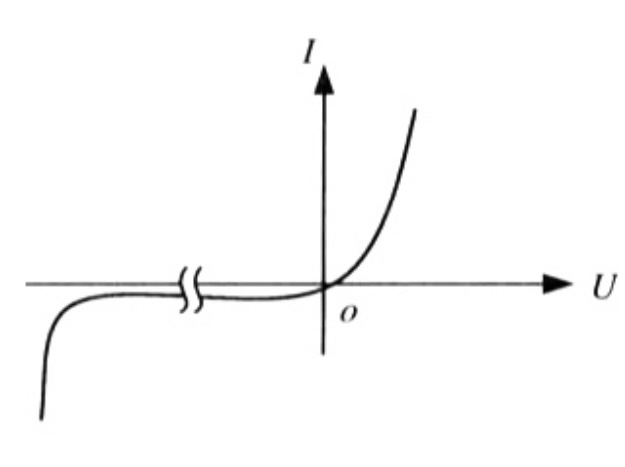
\includegraphics[width = 0.25\textwidth]{二极管}}
		\caption{二极管的伏安特性曲线}
		\label{fig:property1}
	\end{wrapfigure}
	
	
	二极管两端的电压和流过二极管的电流之间的关系如图\ref{fig:property1}所示,在反向击穿前与PN结的伏安关系式$I=I_s(e^{\frac{qU}{kT}}-1)$ ($I_s$为反向饱和电流)基本相同。当二极管两端加正向电压达到某一数值(阀电压),正向电流才开始显著增加。二极管家反向电压时,反向饱和电流很小,当反向电压超过某一个值(反向击穿电压),二极管会发生反向击穿,反向电流剧增,极易烧坏。
	
	\subsubsection{稳压二极管的伏安特性}
	
	\begin{wrapfigure}{1}[1cm]{0pt}
		\fbox{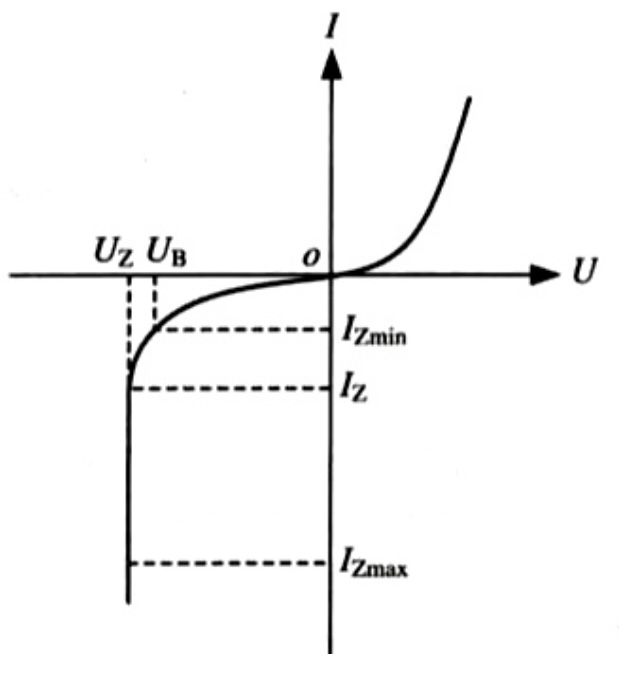
\includegraphics[width = 0.25\textwidth]{稳压管}}
		\caption{二极管的伏安特性曲线}
		\label{fig:property2}
	\end{wrapfigure}



	当二极管两端的反向电压超过击穿电压时,流过二极管的电流急剧增大,而此时管子的端电压变化很小(如图\ref{fig:property2}所示),具有稳压的功能
	

	
	
	\subsection{整流滤波电路}
	如图 \ref{fig:SVCsim}为最简单的整流电路,其中包含一个二极管与负载电阻$R_L$,当正板周期时,二极管导通,负半周时,二极管截止。
	由此达到整流目的,其输出波形如图右侧所示。
	\begin{figure}[htbp]
		\centering
		\fbox{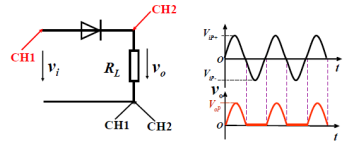
\includegraphics[width=0.5\linewidth]{exp01.jpg}}
		\caption{整流电路电路与波形示意图}
		\label{fig:SVCsim}
	\end{figure}
	则理论上可以计算出输出电压的平均值为
	\begin{equation}
		\bar{V}_0=\frac{1}{T}\int_0^Tv_0(t)dt=\frac{V_p}{\pi}\approx0.318V_p
		\label{eqa:avgV_SVC}
	\end{equation}
	当并联电容时,电容的阻抗随频率增大而减小,因此可以起到一定的滤高频波的作用,其电路图及波形如图 \ref{fig:SVCcom}所示。
	\begin{figure}[htbp]
		\centering
		\fbox{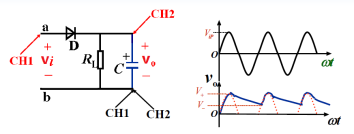
\includegraphics[width=0.5\linewidth]{exp02.png}}
		\caption{整流滤波电路电路与波形示意图}
		\label{fig:SVCcom}
	\end{figure}
	
	\subsection{钳位电路}
	其电路与波形如图 \ref{fig:clamper}所示。二极管作理想处理,当输入正弦波时,当$V_i$上升到$E$时,二极管D导通,$V_o$就不可能再上升,被钳位
	在这一电平上。$V_i$继续上升,多余的电压被充到电容C上,由于二极管正向导通电阻很小,充电很快,电容电压可充到$V_p-E$。
	当$V_i$电压从峰值下降时,二极管截止,输出电压$V_o$为电容上电压和$V_i$的代数和。整个波形被压下$V_p-E$伏,顶端被钳制在E上。
	但实际上二极管有压降,实际分析时需要考虑二极管压降。
	\begin{figure}[htbp]
		\centering
		\fbox{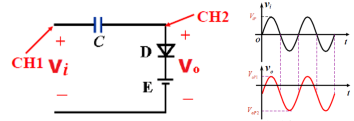
\includegraphics[width=0.5\linewidth]{exp03.png}}
		\caption{钳位电路电路电路与波形示意图}
		\label{fig:clamper}
	\end{figure}
	
	\subsection{限幅电路}
	限幅电路,又称削波电路,是用来限制输出信号电压范围的电路,仅有上门限的称为上限幅
	电路,仅有下门限的称为下限幅电路,具有上下门限的限幅电路,称为双向限幅电路。其工作原理与整流电路相近,由于恒压源的存在,使得当输入电压加上恒压源一旦超出了二
	极管的导通范围,就会截止,因此具有限制幅度的功能。其电路与输出波形如图 \ref{fig:limiter}所示。二极管作理想处理,当输入正弦波时,输出波形最大值受到限制,相当于顶端被“削平”。
	\begin{figure}[htbp]
		\centering
		\fbox{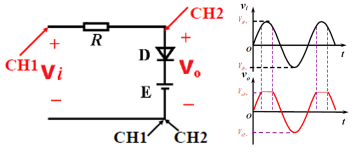
\includegraphics[width=0.5\linewidth]{exp04.png}}
		\caption{限幅电路电路与波形示意图}
		\label{fig:limiter}
	\end{figure}
	
	\subsection{稳压电路}
	其电路图如图 \ref{fig:stabler}所示。当负载$R_L$一定时,如果$V_i$增大,则$V_z$增大,由于稳压二极管动态电阻很小,干路的电流基本上被其捕获,因此$R_1$上的压降增大,最终$V_o$几乎不变。
	当$R_L$减小时,则其干路路电流增大,因此干路压降增大,则$V_z$分压减小,最终$V_o$基本不变。
	\begin{figure}[htbp]
		\centering
		\fbox{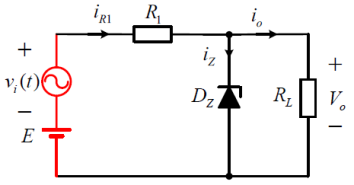
\includegraphics[width=0.5\linewidth]{exp05.png}}
		\caption{限幅电路电路与波形示意图}
		\label{fig:stabler}
	\end{figure}
	
	
	\section{实验内容与步骤}
	\subsection{实验一:整流滤波电路}
	\begin{figure}[H]
		\centering
		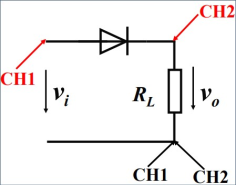
\includegraphics[width=5cm]{exp06.png}
		\caption{实验一电路图}
		\label{fig:Exp1}
	\end{figure}
	如图\ref{fig:Exp1}所示为整流电路。用万用表的两个CH测量其输入和输出电压,再用万用表手动1V DCV档测量其平均值。
	\begin{figure}[H]
		\centering
		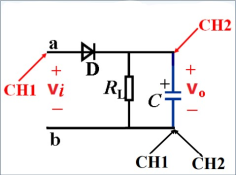
\includegraphics[width=5cm]{exp07.png}
		\caption{实验一(续)电路图}
		\label{fig:Exp1Con}
	\end{figure}
	如图\ref{fig:Exp1Con}所示,在图\ref{fig:Exp1}基础上再并联一个电容$C=10\mathrm{\upmu F}$。用示波器测出其输入、输出电压,再用万用表ACV档测量其纹波电压。然后将电容值改为$C=100\mathrm{\upmu F}$,重复实验。
	\subsection{实验二:钳位电路}
	\begin{figure}[H]
		\centering
		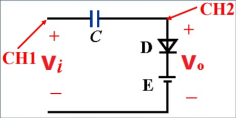
\includegraphics[width=5cm]{exp08.png}
		\caption{实验二电路图}
		\label{fig:Exp2}
	\end{figure}
	如图\ref{fig:Exp2}所示为钳位电路。用示波器测量其输入与输出电压。
	\subsection{实验三:限幅电路}
	\begin{figure}[H]
		\centering
		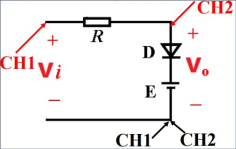
\includegraphics[width=5cm]{exp09.png}
		\caption{实验三电路图}
		\label{fig:Exp3}
	\end{figure}
	如图\ref{fig:Exp3}所示为限幅电路。用示波器测量其输入与输出电压。再用示波器的$X - Y$模式测量其$v_i - v_o$曲线。
	\subsection{实验四:稳压电路}
	\begin{figure}[H]
		\centering
		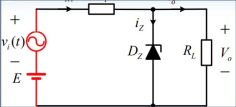
\includegraphics[width=5cm]{exp10.png}
		\caption{实验四电路图}
		\label{fig:Exp4}
	\end{figure}
	如图\ref{fig:Exp4}所示为稳压电路。用示波器测量其输入与输出电压。稳压管等效的交流小信号模型为一个小电阻,用万用表间接测量其等效电路电阻,同时稳压管在静态工作点有一电压降,因此可认为是一反向直流电压源。因此稳压管的等效电路模型是一个小电阻与一个反向直流电源串联。
	
	\section{实验数据处理与分析}
	
	\subsection{实验一:整流滤波电路}
	\begin{figure}[H]
		\centering
		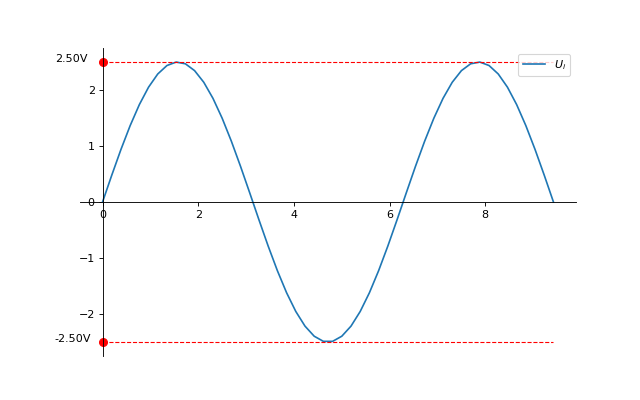
\includegraphics[width=7cm]{Ui.png}
		\caption{实验一输入波形}
		\label{fig:Exp1i}
	\end{figure}
	在未接电容时,输入波形的高峰值为$V_H=2.5\mr{V}$,低峰值为$V_L=-2.50\mr{V}$,如图\ref{fig:Exp1i}所示。
	\begin{figure}[H]
		\centering
		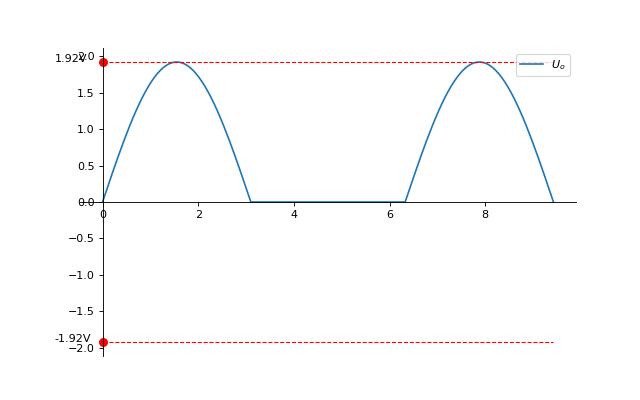
\includegraphics[width=7cm]{U1.png}
		\caption{实验一输出波形}
		\label{fig:Exp1o}
	\end{figure}
	在未接电容时,输出波形的高峰值为$V_H=1.92\mr{V}$,低值被削平,为$V_L=0\mr{V}$,如图\ref{fig:Exp1o}。
	
	\par 万用表测得的平均值为$0.586\mr{V}$。
	而理论给出的平均值为:
	\[ \bar{V_o}=\frac{1}{T}\int_0^TV_o(t)\dd{t}\approx0.318V_P=0.318\times1.92=0.611\mr{V} \]
	\par 这个值比实验值大。分析其原因:万用表可能是测量若干个断点的值,并对对应时间内的电压作近似积分。而万用表的采样频率可能没有快到可以精确测量电压平均值,所以在用矩形分割法进行近似积分时有误差。
	\begin{figure}[H]
		\centering
		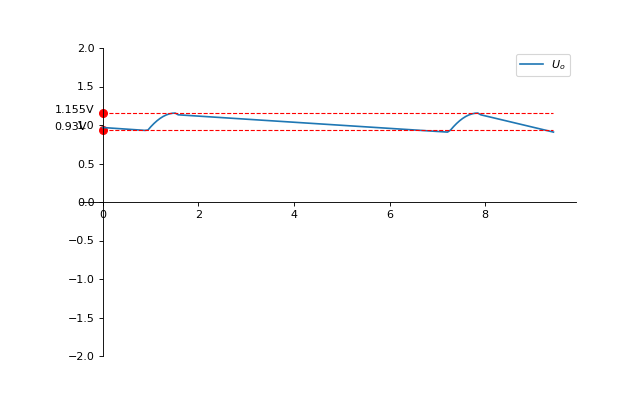
\includegraphics[width=10cm]{U2.png}
		\caption{实验一(续)输出波形,$C=10\mr{\upmu F}$}
		\label{fig:Exp1Cono1}
	\end{figure}
	在电容为$10\mr{\mu F}$时,输出波形如图\ref{fig:Exp1Cono1}所示。其中波纹高值为$V_H=1.155\mr{V}$,波纹低值为$V_L=0.930\mr{V}$。
	\par 万用表测量的平均值为$\widetilde{V_o}=0.0654\mr{V}$。
	\begin{figure}[H]
		\centering
		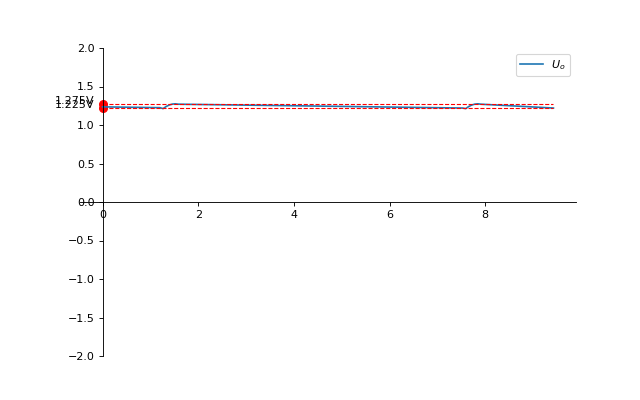
\includegraphics[width=10cm]{U3.png}
		\caption{实验一(续)输出波形,$C=100\mr{\upmu F}$}
		\label{fig:Exp1Cono2}
	\end{figure}
	在电容为$100\mr{\mu F}$时,输出波形如图\ref{fig:Exp1Cono2}所示。其中波纹高值为$V_H=1.275\mr{V}$,波纹低值为$V_L=1.225\mr{V}$。
	\par 万用表测量的平均值为$\widetilde{V_o}=7.368\mr{mV}$。
	\par 比较不同电容值下的结果,我们发现:如果提高电容,那么波纹高值会下降,波纹低值会上升,二者之间差距缩小,所以交流波纹电压减小。
	\par 分析其原因:若电容$C=100\mr{\upmu F}$,那么相较于$C=10\mr{\upmu F}$时,电容的阻抗更小了,与负载电阻的并联阻抗也变小了,分压能力减弱,所以波纹高值减小了;而此时电路的时间常数$\tau=RC$更大了,电路中电压的变化更为缓慢,于是第二次实验的波纹更小,因此波纹低值也更高,交流波纹电压更小。
	\subsection{实验二:钳位电路}
	\begin{figure}[H]
		\centering
		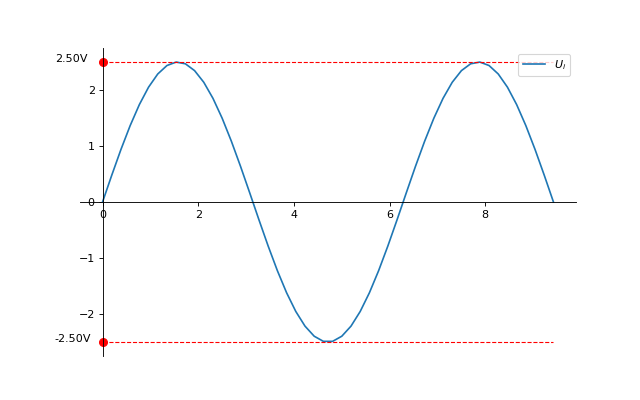
\includegraphics[width=7cm]{Ui.png}
		\caption{实验二输入波形}
		\label{fig:Exp2i}
	\end{figure}
	实验输入波形如图\ref{fig:Exp2i}所示。高峰值为$V_H=2.50\mr{V}$,低峰值为$V_L=-2.50\mr{V}$。
	\begin{figure}[H]
		\centering
		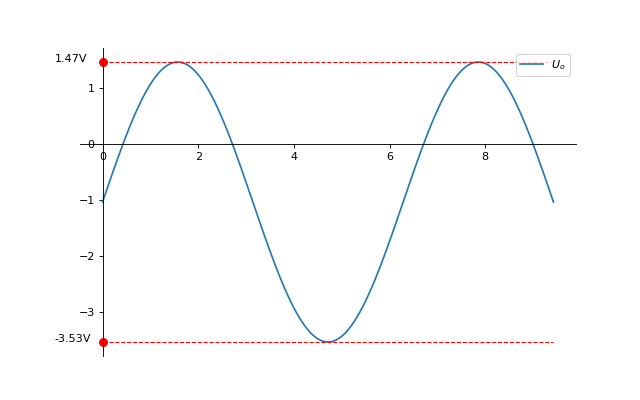
\includegraphics[width=7cm]{U4.png}
		\caption{实验二输出波形}
		\label{fig:Exp2o}
	\end{figure}
	实验输出波形如图\ref{fig:Exp2o}所示。高峰值为$V_H=1.47\mr{V}$,低峰值为$V_L=-3.53\mr{V}$。
	\par 理论上,输出波形相对于输入波形向下平移了$E=1.00\mr{V}$,实际上波形的高峰和低峰分别向下平移了$2.45-1.43=1.03\mr{V}$和$-2.58-(-3.66)=1.03\mr{V}$,和理论值符合得比较好。
	\subsection{实验三:限幅电路}
	\begin{figure}[H]
		\centering
		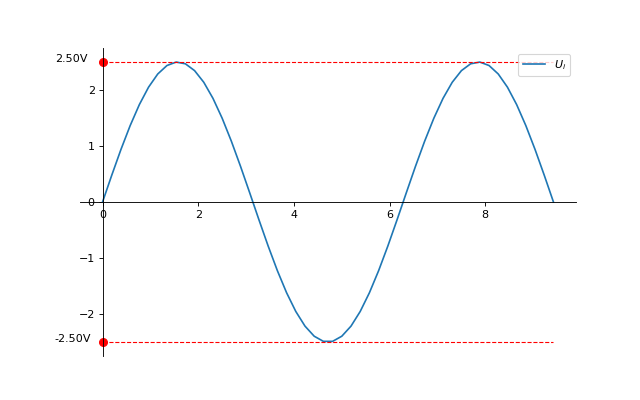
\includegraphics[width=7cm]{Ui.png}
		\caption{实验三输入波形}
		\label{fig:Exp3i}
	\end{figure}
	实验输入波形如图\ref{fig:Exp3i}所示。高峰值为$V_H=2.50\mr{V}$,低峰值为$V_L=-2.50\mr{V}$。
	\begin{figure}[H]
		\centering
		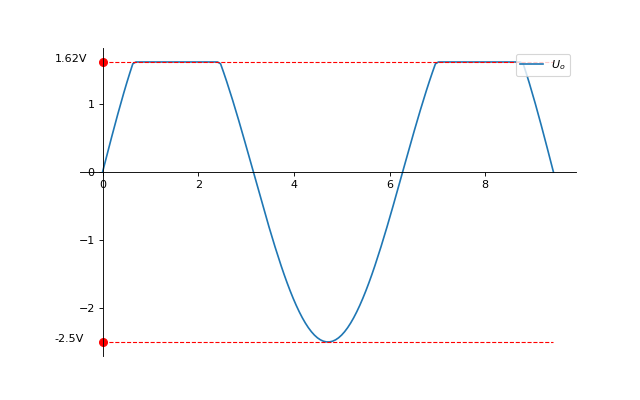
\includegraphics[width=7cm]{U5.png}
		\caption{实验三输出波形}
		\label{fig:Exp3o}
	\end{figure}
	实验输出波形如图\ref{fig:Exp3o}所示。高值被削平,为$V_H=1.62\mr{V}$,低峰值为$V_L=-2.50\mr{V}$。

	\par 将示波器输出模式改为$x - y$模式,测量$v_o - v_i$曲线。
	\begin{figure}[H]
		\centering
		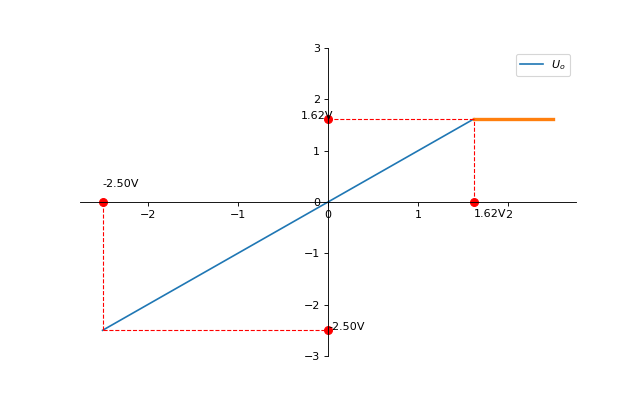
\includegraphics[width=6cm]{U6.png}
		\caption{实验三输出波形,$x - y$模式}
		\label{fig:Exp3oxy}
	\end{figure}
	输出图像如图\ref{fig:Exp3oxy}所示。可见在$u_i$小于阈值电压$1.62\mr{V}$时,$u_o$与$u_i$呈线性关系。若$u_i$大于阈值电压,那么$u_o$被限幅,$u_o$电压值不会继续上升,图线保持水平。
	\subsection{实验四:稳压电路}
	直流电压源$E=12\mr{V}$,接好电路连线再调整函数信号发生器的取值。调整至万用表测量值为$100.09\mr{mV_{rms}}$时,函数信号发生器的标示有效值为$106\mr{mV_{rms}}$。
	\par 改变万用表表笔所接位置,测得稳压管的静态反向电压为$V_Z=5.9974\mr{V_{rms}}$,$R_1$两端电压为$V_1=89.2\mr{mV_{rms}}$,负载电阻$R_L$两端电压为$V_L=2.199\mr{mV_{rms}}$。
	\par 由此计算:
	\[ I_1=\frac{V_1}{R_1}=\frac{89.2\mr{mV}}{1\mr{k}\Omega}=89.2\mr{\upmu A},~
	I_L=\frac{V_L}{R_L}=\frac{2.199\mr{mV}}{2\mr{k}\Omega}=1.0995\mr{\upmu A}.
	\]
	\[
	I_Z=I_1-I_L=88.1\mr{\upmu A},~r=\frac{V_L}{I_Z}=24.96\Omega.
	\]
	得到稳压管的近似等效电阻值
	
	\section{实验总结}
	本次实验着重于二极管的性质和应用。经过若干个二极管实验,我们对二极管的整流、钳位、限幅(削波)有了更深入的认识。同时我们亲手验证了稳压二极管的稳压作用,并用交流小信号模型去求其等效电路。
	\par 在任何规模的电路当中,二极管都是重要的组成成分,所以了解二极管的性质和常见用途,能有效地帮助我们理解复杂电路和自行设计电路。
	
	\section{实验思考题}
	\subsection{设计一个全波整流电路并定性分析说明}
	在原有的半波整流电路的基础上,我们并联另外一组二极管如手绘右图(python实在画不动了)所示。
	其输出到电容器上的波形如图22所示
	\begin{figure}[H]
		\centering
		\fbox{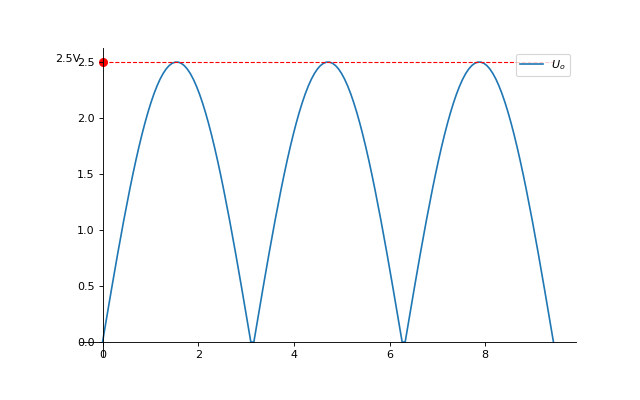
\includegraphics[width=6cm]{U7.png}}
		\caption{全波整流电路电容两端电压特性曲线}
		\label{fig:additional1}
	\end{figure}

	由实验一的原理我们知,可以选取较大的电容值,使并联输出电压的波纹平均值变小,得到较好的全波整流输出。
	
	\subsection{在稳压管电路实验中,电阻R1在电路中的作用}
	提供额外电阻进行分压。
	
	当负载 RL 一定时,如果 Vi 增大,则 Vz 增大,由于稳压二极管动态电阻
	很小,干路的电流基本上被其捕获,因此 R1 上的压降增大,最终 Vo 几乎不变。当 RL 减
	小时,则干路路电流增大,因此干路压降增大,则 Vz 分压减小,最终 Vo 基本不变。反之
	亦然。
	
	假如电路不接入RL,则电路的全部电压加在稳压管的并联支路上,使得稳压管的电压始终为一恒定值,无法研究稳压管在外接电压不同时稳定电压的能力。
	
	\subsection{设计一个电路测量出二极管的伏安特性曲线,画出实验电路图,简明扼要写出实验步骤}
	电路设计如图23所示
	\begin{figure}[H]
		\centering
		\fbox{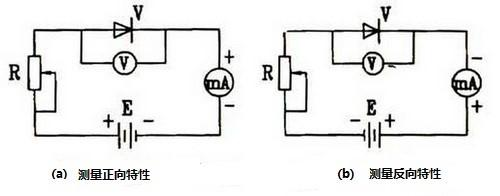
\includegraphics[width=6cm]{特性曲线测量电路.jpg}} 
		\caption{伏安特性曲线测量电路}
		\label{additional2}
	\end{figure}
	其中,图a为正向特性曲线测量电路,图b为正向特性曲线测量电路。
	
	测量时,选取适当的偏置电压,调节滑动变阻器,分别通过电流表和电压表来读取多组电流、电压点,并且在图上进行平滑绘制拟合,即可得到二极管的大致伏安特性曲线图。
	
\end{document}